\documentclass[12pt, letterpaper]{report}
\usepackage{graphicx}
\usepackage{wrapfig}
\usepackage{enumitem}
\usepackage{titlesec}
\usepackage{xcolor}
\usepackage{wrapfig}
\usepackage{ragged2e}
\usepackage{hyperref}
\usepackage[%
    left=1.3in,%
    right=1.3in,%
    top=1.0in,%
    bottom=1.0in,%
    paperheight=11in,%
    paperwidth=8.5in%
]{geometry}%
\definecolor{chaptercolor}{RGB}{27,119,148}
\definecolor{sectioncolor}{RGB}{41,125,139}
\definecolor{subsectioncolor}{RGB}{109,158,108}
\definecolor{textcolor}{RGB}{40,40,40}
\hypersetup{
    colorlinks=true,
    linkcolor=black,
    filecolor=magenta,      
    urlcolor=sectioncolor,
    pdftitle={Overleaf Example},
    pdfpagemode=FullScreen,
    }
\DeclareUnicodeCharacter{202F}{\,}
\graphicspath{{images/}}
\begin{document}
\title{
\begin{picture}(0,0)
\put(-50,200){
\includegraphics[width=4cm]{he2b}}
\end{picture}
La base de données Apache Cassandra}
\author{Costil Iuliana, Hadj Youssef Nader}
\date{Mai 2023}
\maketitle
\tableofcontents
\titleformat{\chapter}
  {\normalfont\LARGE\bfseries\centering\color{chaptercolor}}{\thechapter}{1em}{}
\titleformat{\section}
{\normalfont\Large\bfseries\raggedright\color{sectioncolor}}{\thesection}{1em}{}
\titleformat{\subsection}
{\normalfont\large\bfseries\raggedright\color{subsectioncolor}}{\thesubsection}{1em}{}
\color{textcolor}
\chapter{Introduction à la base de données Cassandra}
\justifying
\section{Présentation de Cassandra}
\textbf{Une base de données NoSQL} (pas seulement SQL) est un type de système de gestion de base de données qui utilise des techniques non tabulaires, orientées document ou clé-valeur pour stocker et récupérer des données. Les bases de données NoSQL sont conçues pour gérer de grandes quantités de données non structurées ou semi-structurées, telles que les publications sur les réseaux sociaux, les données de capteurs et le contenu généré par les utilisateurs.\newline
L'objectif principal d'une base de données NoSQL est de fournir une conception simple, une mise à l'échelle horizontale et un meilleur contrôle de la disponibilité.
\newline
Les exemples de bases de données NoSQL populaires incluent MongoDB, Cassandra, Couchbase et Amazon DynamoDB.
\newline
\underline{\textbf{Apache Cassandra}} est une base de données NoSQL très flexible conçue pour gérer de gros volumes de données sur des clusters de serveurs. Elle a été créée pour répondre aux exigences de performance et de disponibilité des applications Web modernes nécessitant un accès rapide aux données.\newline
Contrairement aux architectures de bases de données relationnelles traditionnelles, Cassandra utilise un modèle de données basé sur des colonnes plutôt que sur des lignes, permettant un stockage efficace de grands ensembles de données avec des modèles de données flexibles et extensibles. Elle est également destinée à être tolérante aux pannes et distribué sur plusieurs nœuds, garantissant que les données restent accessibles même en cas de défaillance d'un nœud.
\newline
Lorsqu'il est nécessaire de stocker des données telles que des profils d'utilisateurs, une messagerie en temps réel, des recommandations de produits, etc., Apache Cassandra reste un très bon choix. De plus, elle travaille dans des domaines tels que la finance, les télécommunications, les réseaux sociaux et la santé. 
\newline
Grâce à ces atouts, Apache Casssandra est devenue une option populaire pour les applications web de nos jours.

\section{Modèles des données utilisées dans Cassandra}
\justifying
Pour apprendre Cassandra, il peut être utile de suspendre temporairement toutes vos connaissances sur le monde relationnel. Nous utilisons une approche ascendante pour comprendre le modèle de données Apache Cassandra. Commençons d'abord par une structure de carte:

\begin{center}
	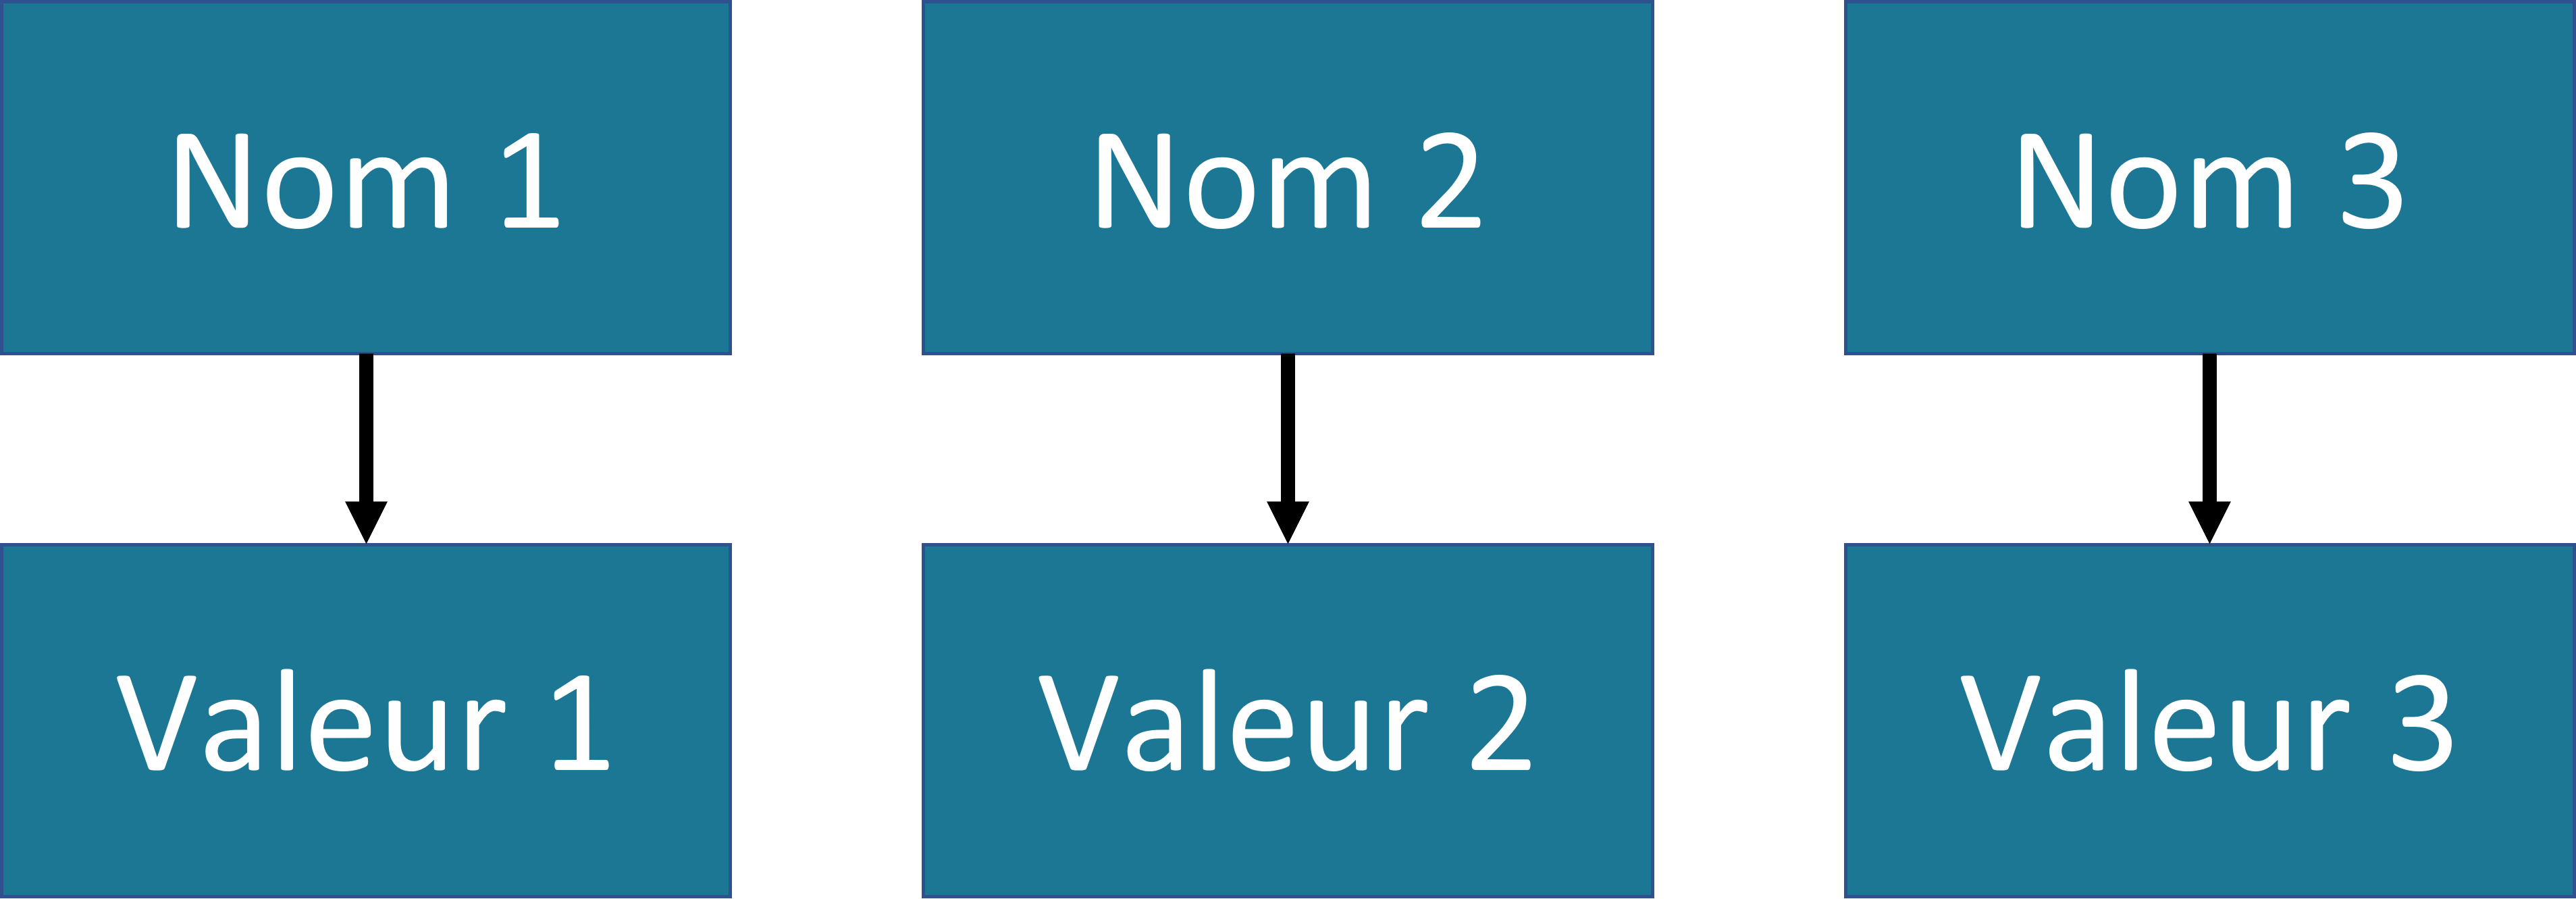
\includegraphics[width=0.6\textwidth]{carte}
\end{center}

\justifying
Cependant, cette structure ne fonctionne que pour une instance d’une entité donnée. Par conséquent, nous avons besoin des lignes pour regrouper les valeurs de colonnes ensemble et des clés de ligne (également appelées clés de partition) pour identifier chaque ensemble de colonnes. Une entité individuelle avec un ensemble de colonnes est appelée une ligne et chaque paire nom-valeur est appelée une colonne.
\begin{center}
	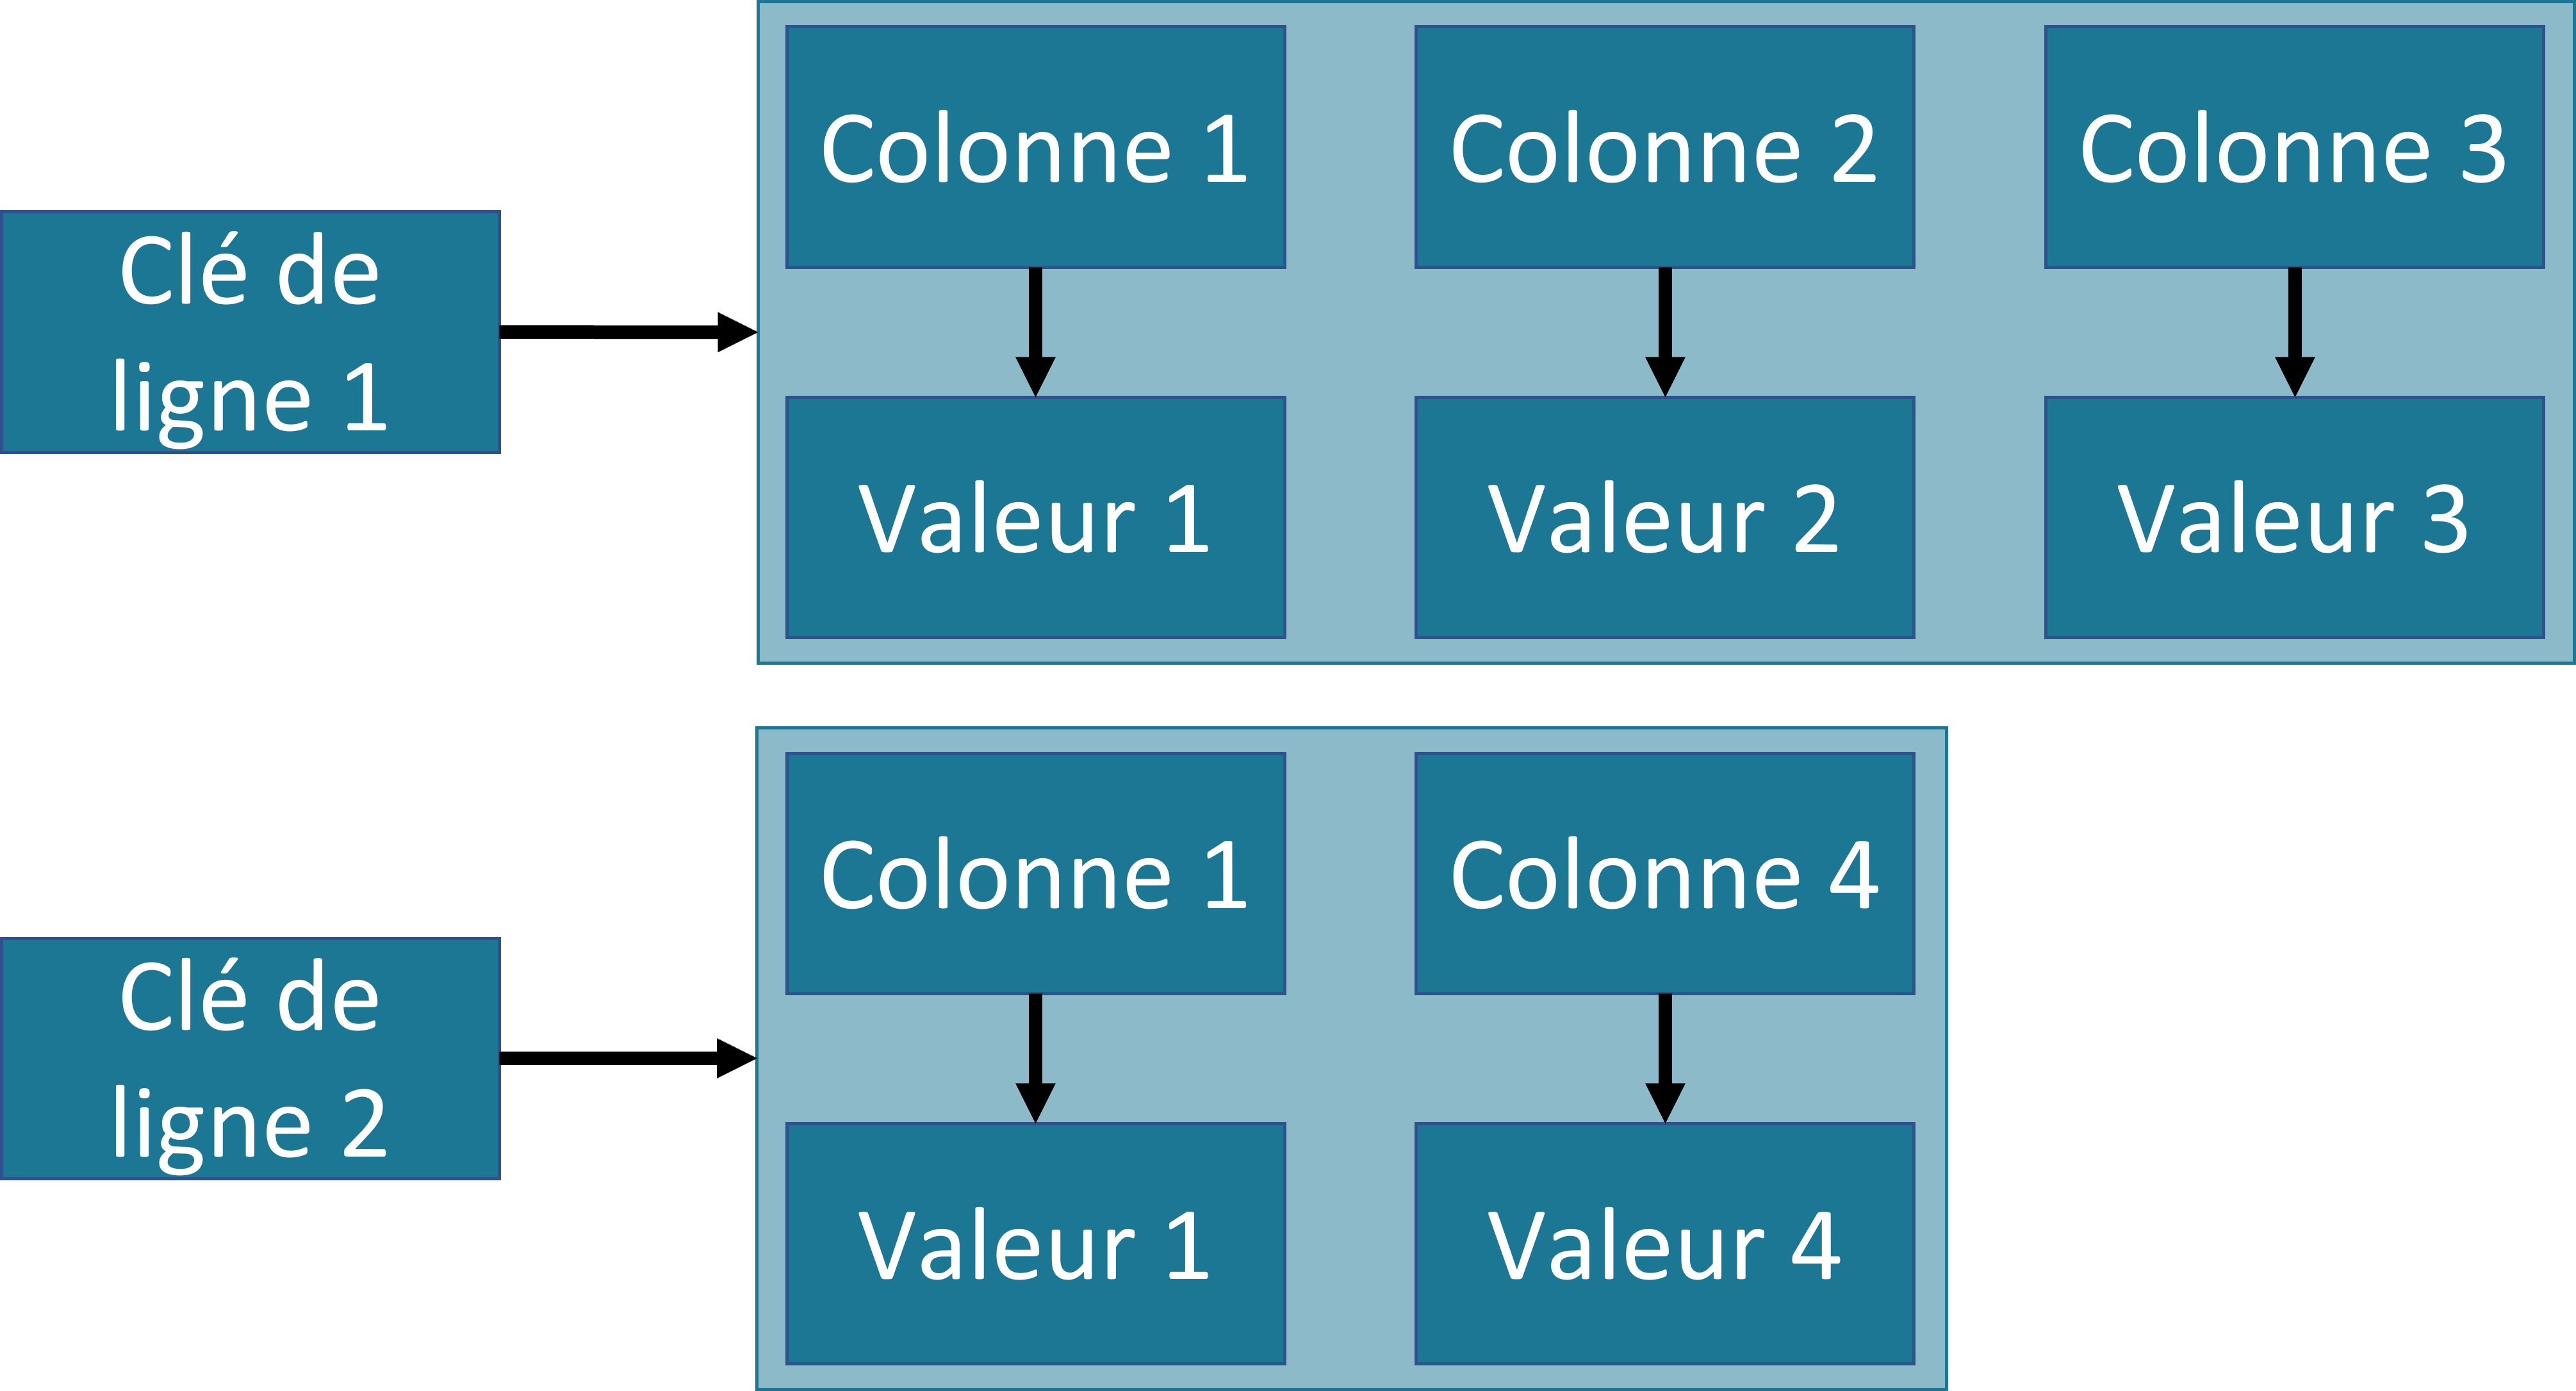
\includegraphics[width=0.8\textwidth]{columnfam}
\end{center}

\subsection{Familles de colonnes }
Apache Cassandra définit une famille de colonnes comme une division logique qui associe des données similaires. Par exemple, nous pourrions avoir une famille de colonnes Utilisateur, une famille de colonnes Hôtel, une famille de colonnes Carnet d'adresses, et ainsi de suite. Ainsi, une famille de colonnes est quelque peu semblable à une table dans le monde relationnel. Les structures de données de base de Cassandra sont les colonnes, qui sont des paires nom/valeur, et la famille de colonnes, qui est un conteneur pour les lignes qui ont des ensembles de colonnes similaires, mais pas identiques. 
\newline
Dans les bases de données relationnelles, nous avons l'habitude de stocker les noms de colonnes uniquement en tant que chaînes - c'est tout ce qui est autorisé. Mais dans Cassandra, nous n'avons pas cette limitation. Les clés de ligne et les noms de colonnes peuvent être des chaînes, comme les noms de colonnes relationnels, mais ils peuvent également être des entiers longs, des UUID ou tout type de tableau de bytes. Cela révèle une autre qualité intéressante des colonnes de Cassandra : elles ne doivent pas être aussi simples que des paires nom/valeur prédéfinies ; vous pouvez stocker des données utiles dans la clé elle-même, pas seulement dans la valeur. 
\newline
De plus, vous n'avez pas besoin d'enregistrer une valeur pour chaque colonne chaque fois que vous enregistrez une nouvelle entité. Parfois, vous ne connaissez pas la valeur de chaque colonne pour une entité particulière. Par exemple, certains ont un deuxième numéro de téléphone et d'autres non. De plus, les formulaires en ligne soutenus par Apache Cassandra ont des champs qui sont facultatifs et d'autres qui sont obligatoires. Au lieu de stocker null pour les valeurs inconnues qui gaspillent de l'espace, nous ne stockons tout simplement pas cette colonne pour cette ligne.
\newline
Il peut être utile de penser à cela en termes de JavaScript Object Notation (JSON). 


\begin{center}
	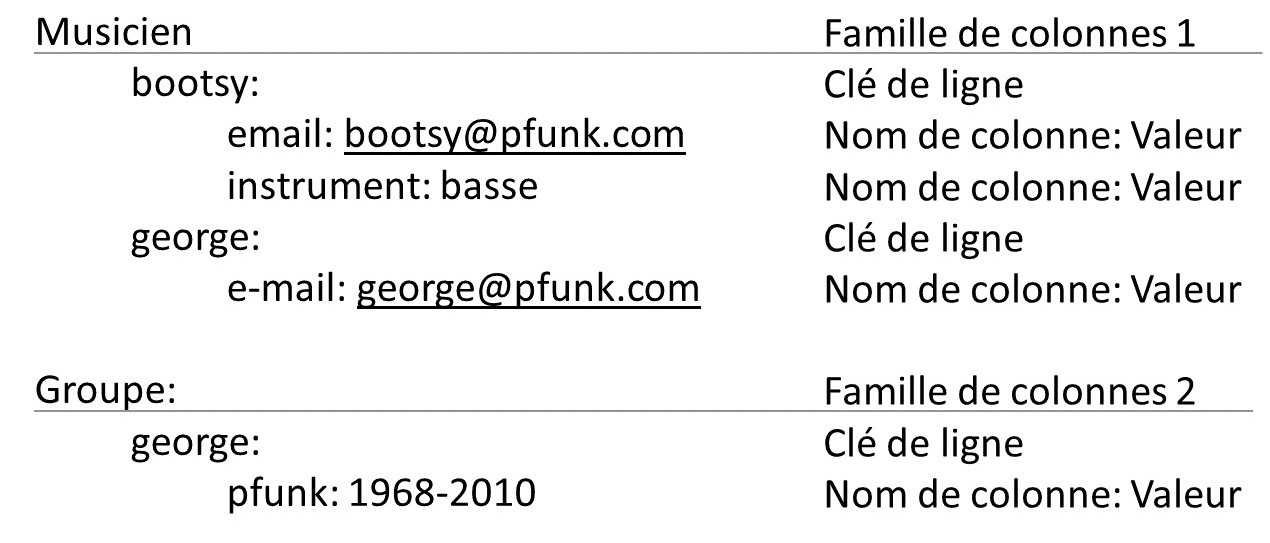
\includegraphics[width=\textwidth]{json}
\end{center}

Voici deux familles de colonnes, Musicien et Groupe. La famille de colonnes Musicien contient deux rangées, "bootsy" et "george". Ces deux rangées ont un ensemble irrégulier de colonnes associées: le dossier bootsy a deux colonnes (email et instrument) et le dossier george n'a qu'une seule colonne. Dans Cassandra, c'est normal. La deuxième famille de colonnes est Groupe et elle a également une rangée "george" avec une colonne nommée "pfunk".
\newline
Et si nous voulions créer un groupe de colonnes liées, c'est-à-dire ajouter une autre dimension à cela? Cassandra nous permet de le faire avec quelque chose appelé une super famille de colonnes. Une super famille de colonnes peut être considérée comme une carte de cartes.

\begin{center}
	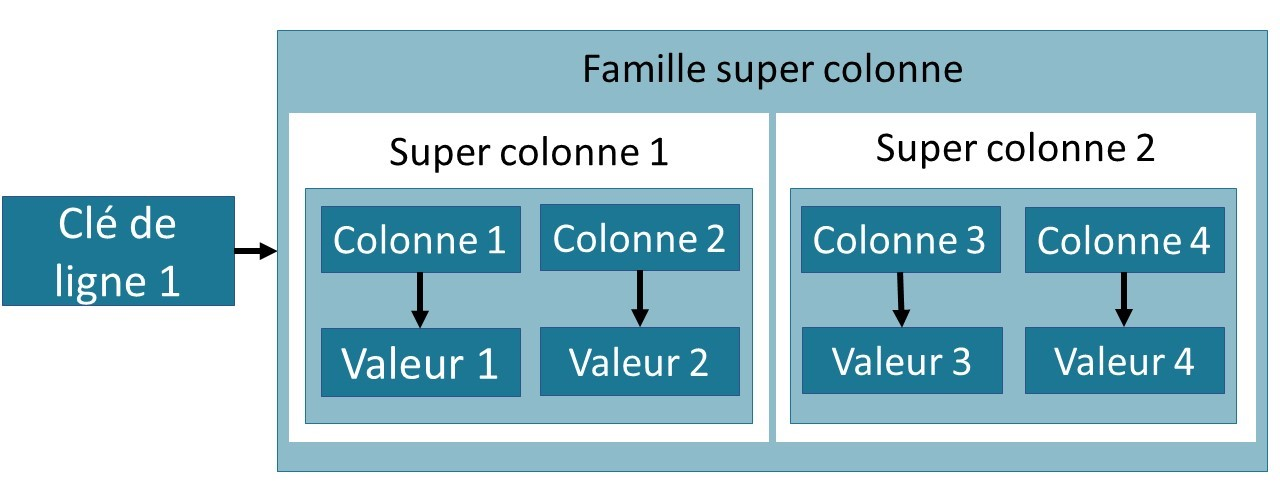
\includegraphics[width=\textwidth]{supercolumnfam}
\end{center}

L'adresse d'une valeur dans une famille de colonnes régulière est une clé de ligne pointant vers un nom de colonne pointant vers une valeur, tandis que l'adresse d'une valeur dans une famille de colonnes de type "super" est une clé de ligne pointant vers un nom de colonne pointant vers un nom de sous-colonne pointant vers une valeur. 
\newline
\subsection{Keyspace: le conteneur logique des familles de colonnes}
Le conteneur de données fondamental dans Apache Cassandra est le keyspace, qui est parfois comparé à une base de données dans un système de gestion de base de données relationnelle, malgré des différences considérables. Par exemple, un keyspace, contrairement à une base de données relationnelle, n'applique pas de schéma fixe pour les données stockées dans des tables. Les tables d'un keyspace peuvent avoir des schémas différents et être optimisées pour diverses charges de travail.
\newline
Il est courant de créer un keyspace par application, mais il est possible de créer autant de keyspaces que vous en avez besoin. Cependant, la création de centaines de keyspaces par application peut générer des problèmes. Un seul keyspace fonctionne généralement sur un cluster, mais plusieurs peuvent y fonctionner sous certaines conditions de sécurité et de partitionnement.
\newline
À l'intérieur d'un keyspace se trouvent une ou plusieurs familles de colonnes. Il possède un nom ainsi qu'un ensemble d'attributs qui décrivent son comportement. Les attributs de base que vous devez définir lors de la création d'un keyspace sont: la stratégie de placement des répliques et le facteur de réplication (qu’on va detailler plus tard).


\chapter{Architecture et mechanismes utilisées dans Cassandra}
\section{Vue d'ensemble de l'architecture de Cassandra}
L'architecture de Cassandra est conçue pour offrir une haute disponibilité, une évolutivité horizontale et une tolérance aux pannes. Elle est basée sur un modèle de cluster distribué qui répartit les données sur plusieurs nœuds afin de garantir la résilience, la flexibilité et la performance de la base de données. Cassandra suit une approche "peer-to-peer" dans laquelle chaque nœud peut accepter des requêtes et est responsable de sa propre gestion.

\begin{center}
	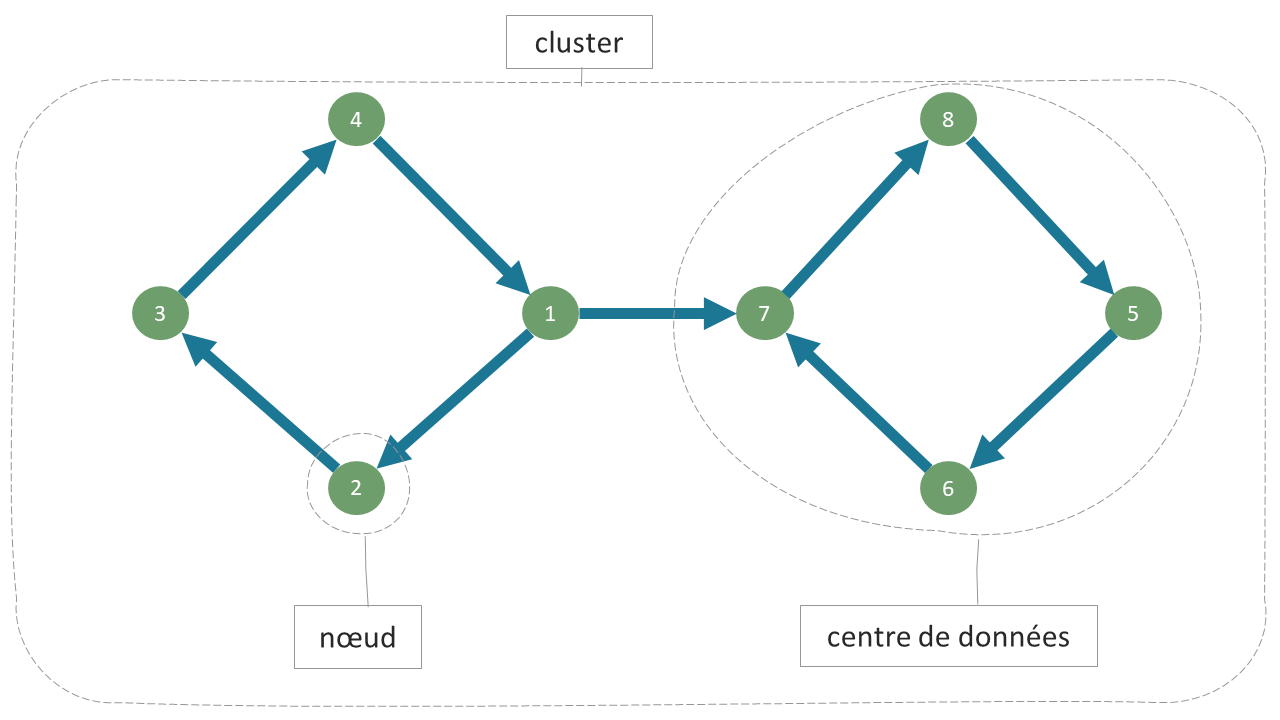
\includegraphics[width=\textwidth]{architecture}
\end{center}
\begin{itemize}
  \item Nœud : Un nœud est l'unité de base de l'architecture de Cassandra. Il s'agit d'un serveur physique ou virtuel qui stocke des données et exécute des opérations de traitement de données. Chaque nœud peut communiquer avec d'autres nœuds via un protocole “gossip” (protocole de ragots) pour assurer la cohérence des données.
  \item Centre des données : Un centre des données est une collection de nœuds associés physiquement proches les uns des autres.
  \item Cluster : Un cluster est un groupe de centre des données avec des nœuds qui travaillent ensemble pour stocker et gérer les données. Les données sont réparties sur plusieurs nœuds dans le cluster, ce qui permet de garantir la disponibilité et la performance de la base de données. Il est parfois appelé anneau puisque Apache Cassandra alloue des données aux nœuds du cluster en les organisant dans un anneau. C’est le phénomène de clustering.
\end{itemize}

En résumé, l'architecture de Cassandra est basée sur un modèle de cluster distribué qui utilise des nœuds pour stocker et gérer les données. Les tables sont utilisées pour stocker les données, et chaque nœud est responsable de la gestion de ses propres données. Cette architecture garantit une base de données populaire pour les applications à grande échelle.

\section{Lecture et écriture des données}
Cassandra fournit une architecture véritablement "indépendante de la localisation" en ce qui concerne la lecture et l'écriture de données. Cela signifie que n'importe quel nœud dans un cluster Cassandra (peu importe si ce nœud fait partie d'une configuration à centre de données unique ou multiple) peut être lu ou écrit indépendamment de l’endroit.
\begin{center}
	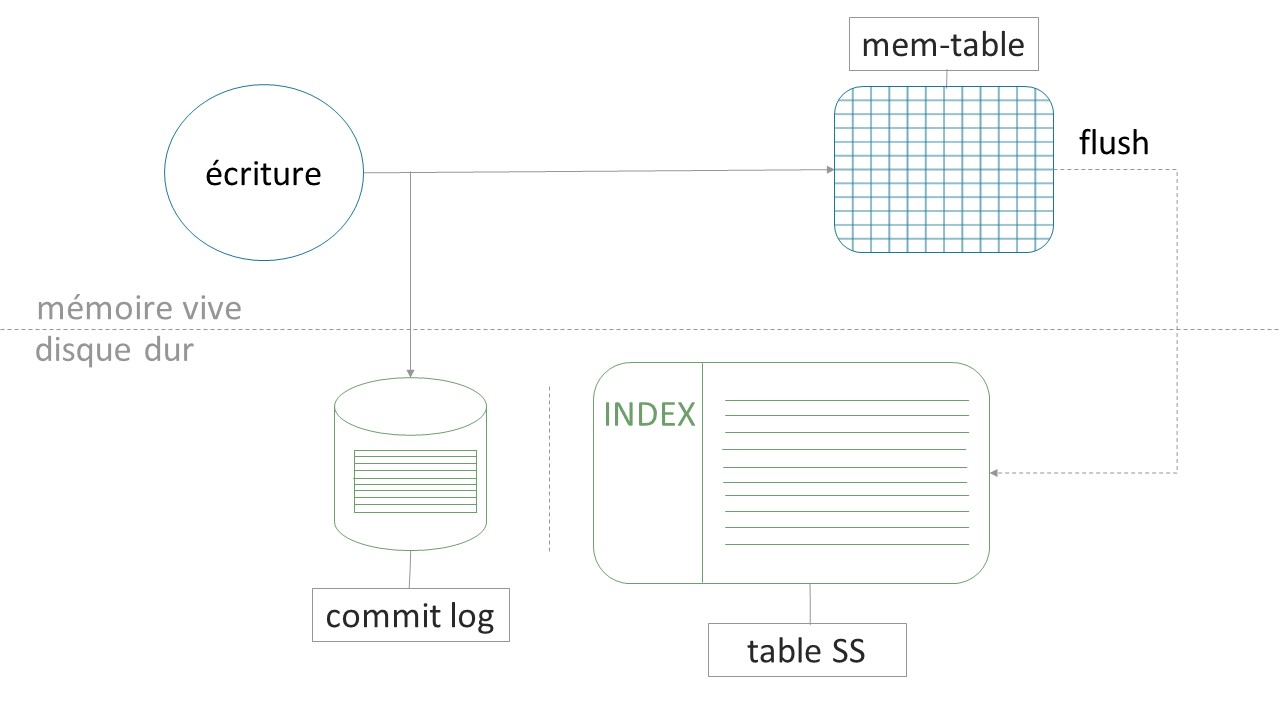
\includegraphics[width=\textwidth]{ecriture}
\end{center}
\begin{itemize}
  \item Commit log : Le commit log est un mécanisme de stockage de secours dans Cassandra qui enregistre toutes les opérations d'écriture avant leur exécution sur la Mem-Table. Le commit log est utilisé pour la récupération de données en cas de défaillance du système ou d'interruption de service.
  \item Mem-Table (Memory Table): La Mem-Table est un composant de la mémoire vive de chaque nœud de Cassandra qui stocke les données en attente d'écriture sur le disque. Elle est organisée en une structure de type arbre pour permettre une recherche rapide et efficace. Lorsque la Mem-Table est pleine, les données sont écrites sur le disque, et la Mem-Table est vidée pour être prête à stocker de nouvelles données.
  \item Table SS (Sorted String Table): La table SS (SSTable) est une structure de données de stockage de Cassandra qui stocke les données de manière permanente sur le disque dur. Elle est optimisée pour permettre une lecture rapide des données, et est utilisée pour stocker les données qui ont été écrites sur la Mem-Table.
\end{itemize}
Lorsque des données sont écrites dans Apache Cassandra, elles sont d'abord écrites dans un commit log, ce qui garantit une durabilité et une sécurité totales des données, qui sont également écrites dans une structure en mémoire appelée "mem-table", qui est finalement vidée dans une structure de disque appelée "table ss" (tableau de chaînes triées).
\newline
Si un ou plusieurs nœuds responsables d'un ensemble de données particulier sont hors service, les données sont simplement écrites sur un autre nœud, qui conserve temporairement les données. Une fois que le(s) nœud(s) sont de retour en ligne, ils se mettent automatiquement à jour à partir des nœuds qui gèrent leurs données stockées en interne. La lecture des données est effectuée en parallèle sur l'ensemble du cluster. Un utilisateur demande des données à n'importe quel nœud (qui devient le nœud coordinateur de cet utilisateur), avec la requête de l'utilisateur étant assemblée à partir d'un ou plusieurs nœuds conservant les données nécessaires. Si un nœud particulier ayant les données requises est en panne, Apache Cassandra demande facilement les données à un autre nœud qui détient une copie répliquée de ces données.

\subsection{"Peer to peer"}
Dans les bases de données traditionnelles qui peuvent être déployées sur plusieurs machines (comme MySQL), et même dans les modèles plus récents tels que le Bigtable de Google, certains nœuds sont désignés "maîtres" et d’autres sont des "esclaves". Ils ont des rôles différents dans le cluster global : le maître agit en tant que source autoritaire des données, et les esclaves synchronisent leurs données avec le maître. Toutes les modifications écrites sur le maître sont transmises aux esclaves. Ce modèle est optimisé pour la lecture de données, car il permet de lire des données à partir de n'importe quel esclave. Mais la réplication est unidirectionnelle, du maître vers l'esclave. Cela a un impact important : toutes les écritures doivent être envoyées au maître, ce qui signifie qu'il peut être un point de défaillance potentiel. Dans une configuration maître/esclave, le nœud maître peut avoir des effets importants s'il est hors ligne.
\newline
En revanche, Cassandra a un modèle de distribution pair à pair, de sorte que chaque nœud donné est structurellement identique à n'importe quel autre nœud - c'est-à-dire qu'il n'y a pas de nœud "maître" qui agit différemment d'un nœud "esclave".
\newline
La conception pair à pair facilite à la fois la mise à l'échelle et la disponibilité générale de la base de données par rapport à la réplication maître/esclave.

\subsection{Le Protocole Gossip}
Le protocole gossip (ou protocole de ragots) est un protocole de communication utilisé dans les systèmes distribués pour assurer la cohérence des données. Il tire son nom de l'idée que les nœuds communiquent des informations à leurs voisins de manière similaire à la façon dont les gens échangent des ragots dans une communauté.
\newline
Dans Apache Cassandra, le protocole gossip est utilisé pour permettre aux nœuds de se découvrir et de se synchroniser entre eux. Chaque nœud maintient une liste des autres nœuds du cluster ainsi que des informations sur leur état et leur santé. Le protocole gossip permet à chaque nœud de diffuser ces informations à ses voisins. De cette façon, toutes les informations sur l'état du cluster se propagent rapidement et efficacement à tous les nœuds.
\newline
Lorsqu'un nœud reçoit des informations, il les utilise pour mettre à jour sa propre vue du cluster. Si les informations sont contradictoires ou incohérentes, le nœud essaie de les résoudre en utilisant des règles de résolution de conflits spécifiques. Par exemple, si deux nœuds annoncent des adresses IP différentes pour un même nœud, le nœud qui a la plus haute adresse IP est considéré comme étant le "vrai" nœud.
\newline
En fait, ce protocole est un élément clé de la robustesse et de la résilience d’Apache Cassandra, qui permet non seulement aux nœuds de se découvrir et de se synchroniser automatiquement mais aussi, il assure que le cluster fonctionne de manière cohérente même en présence de défaillances matérielles ou logicielles.

\chapter{Performance de Cassandra}
\section{Principales caractéristiques et avantages de l'utilisation de Cassandra}
On peut citer:
\subsection{La tolérance aux pannes}
\justifying
Le modèle de distribution pair à pair permet à Apache Cassandra de fournir une distribution automatisée des données sur tous les nœuds à l'intérieur d'un anneau (ring) ou d'un cluster de bases de données. Étant donné de ça, un développeur ou un administrateur ne doit rien faire pour distribuer les données. 
\newline
Apache Cassandra garantit également une réplication personnalisée, qui conserve des copies redondantes des données sur les nœuds du même ring. Cela implique que si un nœud d'un cluster tombe en panne, une ou plusieurs copies des données de ce nœud sont disponibles sur d'autres machines du cluster.
\newline 
Cassandra répartit les répliques de données sur les nœuds en fonction de ces deux approches:
\begin{itemize}
  \item La stratégie de réplication détermine où placer la prochaine réplique.
  \item Le facteur de réplication détermine le nombre total de copies distribuées sur différents nœuds.
\end{itemize}  
\justifying
Un facteur de réplication indique une seule copie de données, tandis que si on a trois, cela implique trois copies de données sur trois nœuds différents. Il s’agit bel et bien d’un nombre qui vaut trois pour s'assurer qu'il n'y aura pas d’échec.
\newline 
Cassandra a deux types de stratégies de réplication:
\newline
\justifying
\textbf{SimpleStrategy: }
\newline
\justifying
Quand on a un seul centre de données, on fait appel à SimpleStrategy qui définit le réplica initial sur le nœud choisi par le partitionneur. Les répliques restantes sont ensuite placées dans le ring des nœuds en respectant le sens des aiguilles d'une montre.
\textbf{NetworkTopologyStrategy: }
\newline
\justifying
Quand on a plus de deux centres de données, le sauveur c’est NetworkTopologyStrategy.
\newline
Les répliques sont configurées indépendamment pour chaque centre de données. Elles se déplacent dans le sens des aiguilles d'une montre autour du ring jusqu'à ce qu'elles atteignent le premier nœud dans une autre étagère. 
\newline
Cette approche tente de les répartir sur plusieurs étagères dans le même centre de données. En effet, des pannes ou des problèmes peuvent se développer dans l’étagère à tout moment mais ces données là peuvent être récupérées via les répliques qui sont stockées sur d'autres nœuds.

\centering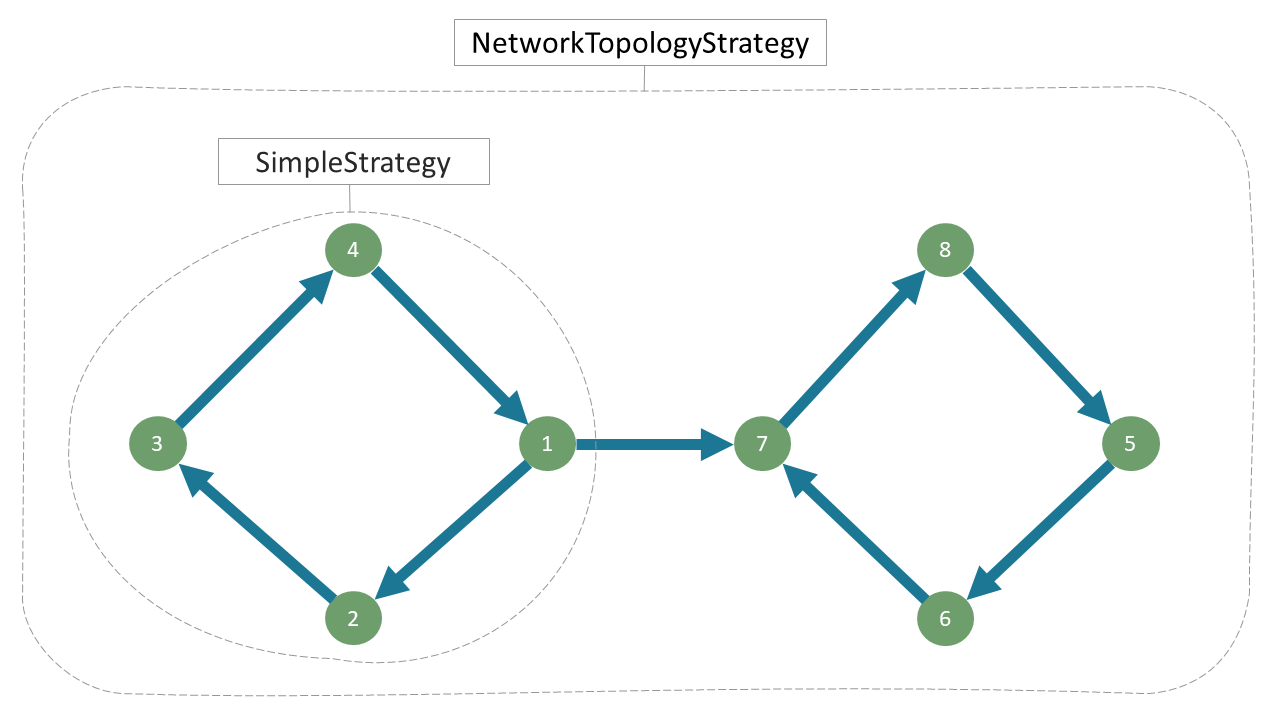
\includegraphics[width=\textwidth]{replicationStrategy}
\subsection{La scalabilité horizontale}
\justifying
La scalabilité est la capacité architecturale d'un système à continuer à traiter plus de demandes avec peu de sacrifices en termes de performances.
\newline
L'un des grands avantages d'Apache Cassandra est l'évolutivité horizontale due à sa structure. Cela permet aux utilisateurs de réagir efficacement en cas d’augmentation soudaine de la demande. Il vous suffit d'ajouter des machines supplémentaires qui contiennent une partie ou la totalité de vos données, et aucune machine n'est responsable de l'intégralité de la charge de travail de traitement des requêtes. De toute évidence, les clusters peuvent facilement évoluer vers le haut et vers le bas grâce à la mise à l'échelle élastique, qui est un sous-ensemble de la mise à l'échelle horizontale.
\newline
Pour ce faire, le cluster doit être en mesure d'accepter de nouveaux nœuds, qui peuvent obtenir des copies de tout ou partie des données et commencer à répondre aux nouvelles demandes des utilisateurs sans interruption majeure ni reconfiguration du cluster. Il n'est pas nécessaire de redémarrer le processus, ni de modifier les requêtes d'application, ni de réaligner manuellement les données.
\newline
Apache Cassandra répond aux exigences d'un système évolutif horizontal idéal en permettant l'ajout de nœuds en toute transparence. Si vous avez besoin de plus de capacité, ajoutez des nœuds au cluster et le cluster utilisera automatiquement les nouvelles ressources. Voilà pourquoi de nombreuses entreprises adoptent cette solution pour le Big Data.

\subsection{La gestion de la disponibilité des données}
Le théorème CAP, également connu sous le nom de théorème de Brewer, stipule qu'un système informatique distribué ne peut pas fournir simultanément les trois garanties suivantes : cohérence (tous les nœuds voient les mêmes données en même temps), disponibilité (chaque requête reçoit une réponse indiquant si la requête a réussi), tolérance pour le partitionnement (le système continue de fonctionner malgré la perte arbitraire de messages ou la défaillance d'une partie du système). 
\newline
La disponibilité est très importante pour les services à forte demande. Une mauvaise disponibilité entraîne une mauvaise expérience utilisateur, l'insatisfaction des consommateurs et des pertes financières. 
\newline
Cassandra est généralement classé comme un système AP (comme de nombreux systèmes de Big Data). En d'autres termes, Cassandra est une base de données qui privilégie la disponibilité à la cohérence (bien que vous puissiez préciser le niveau souhaité lors de la requête grâce au "niveau de cohérence"). 
\newline
Comme mentionné précédemment, la réplication des données permet à Cassandra de conserver des copies redondantes des données sur plusieurs nœuds, garantissant ainsi la disponibilité des données en cas de défaillance d'un nœud ou d'un centre de données entier. De plus, Cassandra utilise une architecture distribuée qui élimine les points de défaillance uniques, ce qui signifie qu'il n'y a pas de nœud maître unique qui pourrait causer une interruption du système en cas de panne. Chaque nœud dans le cluster est également capable de répondre aux demandes des utilisateurs, de sorte que le système est toujours disponible même si un ou plusieurs nœuds échouent. 
\newline
En fin de compte, la tolérance aux pannes est un élément important de la gestion de la disponibilité des données. En cas de défaillance d'un composant, la tolérance aux pannes minimise les temps d'arrêt et maximise  la disponibilité des données. Cependant, la gestion de la disponibilité des données inclut souvent d'autres aspects tels que la sauvegarde, la restauration et la protection des données.

\chapter{Sécurité}

\section{Authentification et Autorisation}
L'authentification et l'autorisation sont des éléments cruciaux pour assurer la sécurité de Cassandra. Bien que les nœuds de Cassandra soient souvent situés derrière des pare-feu, des VPN ou des VPC, les applications qui y accèdent peuvent être vulnérables aux attaques malveillantes.
\newline
Apache Cassandra utilise un mécanisme d'authentification et d'autorisation de sécurité semblable à celui d'un système de gestion de base de données relationnelles (RDBMS). En effet, Apache Cassandra offre un système d'authentification et d'autorisation qui peut être activé en modifiant les paramètres dans le fichier de configuration cassandra.yaml. Les deux paramètres à modifier sont l'authentificateur et l'autorisateur. Par défaut, ces paramètres sont définis sur "AllowAllAuthenticator" et "AllowAllAuthorizer", ce qui signifie que tous les utilisateurs sont autorisés à se connecter à Cassandra sans authentification.
\newline
Cependant, il est fortement recommandé de mettre en place un système d'authentification et d'autorisation solide pour limiter l'accès aux utilisateurs autorisés uniquement. Cassandra propose deux mécanismes de sécurité : PasswordAuthenticator pour l'authentification et CassandraAuthorizer pour l'autorisation. En utilisant ces mécanismes, les administrateurs peuvent restreindre l'accès aux utilisateurs ayant des autorisations spécifiques.
\newline
Il est également important de créer un nouveau super-utilisateur avec un nouveau mot de passe et de supprimer l'utilisateur par défaut lors de la première connexion à Cassandra pour éviter les attaques potentielles. Enfin, pour des besoins de sécurité spécifiques, il est possible de mettre en place son propre système d'authentification et d'autorisation en implémentant les interfaces Iauthenticator pour l'authentification et Iauthorizer pour l'autorisation.

\section{Cryptage de données}
Apache Cassandra dispose de nombreuses méthodes de cryptage des données pour aider à protéger les données de votre base de données contre les accès indésirables.
\newline
\begin{itemize}
  \item Le cryptage côté client est un type de chiffrement de données qui chiffre les données avant qu'elles ne soient stockées dans la base de données. Même si un attaquant parvient à accéder à votre base de données, il ne pourra pas accéder à vos données en clair. Vous pouvez utiliser une bibliothèque cryptographique comme OpenSSL pour implémenter cette procédure, ou vous pouvez configurer un service de gestion de clés comme AWS Key Management Service.
  \item Le cryptage au niveau du cluster est autre option de chiffrement qui peut être activée en configurant les paramètres SSL/TLS de Cassandra. Le chiffrement se produit au niveau du cluster, ce qui implique que les données sont chiffrées pendant leur transit entre les nœuds Cassandra. Cette option garantit que le transfert est terminé et que les données sont envoyées en toute sécurité.
\end{itemize} 
Il convient de noter que l'inclusion de mesures cryptographiques pourrait réduire les performances de Cassandra. Dans ce cas, il est essentiel de sélectionner les options de chiffrement en fonction de l'importance des données contenues dans la base de données et du niveau de protection requis. Nous vous recommandons également de mettre en place un système de gestion des clés solides et d'analyser périodiquement les journaux pour détecter tout comportement inhabituel afin de renforcer la sécurité.

\section{Gestion des certificats}
En plus du cryptage de données, Cassandra offre également la possibilité d'utiliser des certificats pour sécuriser les communications entre les différents nœuds d'un cluster et les clients. Les certificats permettent d'authentifier les nœuds et les clients, empêchant ainsi les attaques de type "Man-in-the-middle". 
\newline
L'utilisation de certificats en Cassandra peut fournir une sécurité accrue lors de la communication entre les différents nœuds d'un cluster et les clients. Les certificats permettent de s'assurer que les communications sont chiffrées et authentifiées, ce qui empêche les attaquants de s'immiscer dans la communication et de modifier les données. Les certificats peuvent être créés à l'aide de services tiers ou générés à l'aide d'un service de gestion de clés tel que AWS Key Management Service, ce qui permet aux organisations de personnaliser la sécurité de leurs clusters en fonction de leurs besoins spécifiques.

\section{Sécurité physique}
La sécurité physique des nœuds Cassandra est également importante pour garantir la confidentialité et l'intégrité des données stockées. Il est recommandé de mettre en place des mesures de sécurité telles que la restriction de l'accès physique aux nœuds, la surveillance de l'environnement (température, humidité, etc.), et la mise en place de systèmes de protection contre les pannes de courant et les incendies.
\newline
La sécurité physique est essentielle pour protéger les nœuds Cassandra contre les menaces physiques telles que le vol, la destruction ou la détérioration des équipements. Pour garantir la sécurité physique, les organisations peuvent restreindre l'accès physique aux nœuds, installer des caméras de surveillance, des détecteurs de mouvement et de fumée, des systèmes de refroidissement et des onduleurs pour protéger les données stockées en cas de pannes de courant. Les organisations peuvent également mettre en place des politiques et des procédures pour s'assurer que les nœuds sont bien protégés et surveillés en permanence.

\chapter{Conclusion}
\section{Cas pratique}
Instagram est l'une des plateformes de réseaux sociaux les plus populaires au monde, avec plus d'un milliard d'utilisateurs actifs mensuels. Pour offrir une expérience utilisateur rapide et fiable, Instagram a besoin d'une base de données qui puisse gérer des quantités massives de données de manière efficace. C'est là que Cassandra entre en jeu et devient officiellement la base de donnée utilisée par Instagram et ça depuis 2012 afin de remplacer Redis et prendre en charge des cas d'utilisation de produits tels que la détection de fraude.
\newline
Le choix de Cassandra est due à plusieurs critères tels que sa capacité à gérer des données semi-structurées et non structurées, sa manière de gérer des requêtes en temps réelle dans le but d'offrir une expérience utilisateur rapide ainsi sa flexibilité dans la gestion des données et son adaptation par rapport aux applications qui nécessitent une haute disponibilité et une tolérance aux pannes puisqu’elle est conçue pour être résiliente aux pannes de serveurs individuels. 
\newline
En revanche, Cassandra permet aussi de fonctionner sur des clusters de serveurs, ce qui signifie qu'elle peut facilement s'étendre à mesure que les besoins de stockage augmentent. Cette architecture distribuée garantit également une haute disponibilité, même en cas de défaillance d'un ou plusieurs serveurs, cela va permettre à Instagram de continuer à fonctionner normalement, sans interruption de service afin d’améliorer la gestion des profils des utilisateurs, faciliter leurs interactions et qu’il pourra stocker une grande variété de données, notamment les commentaires, les likes, les followers, les recherches et les photos.
\newline
Pour stocker ces photos de manière efficace, Instagram utilise une technique appelée "compression de niveau média" qui utilise une combinaison de compression de fichiers JPEG et de compression de données pour stocker les images en Cassandra. Cette technique permet d'économiser de l'espace de stockage sans compromettre la qualité des images.
\newline
Afin de réduire la latence de lecture et d’écriture de Cassandra l'équipe Cassandra d'Instagram a commencé à travailler sur un projet, que nous appelons Rocksandra.
\newline
Ci-joit deux graphes illustratives qui montrent le résultat obtenu :
\begin{center}
	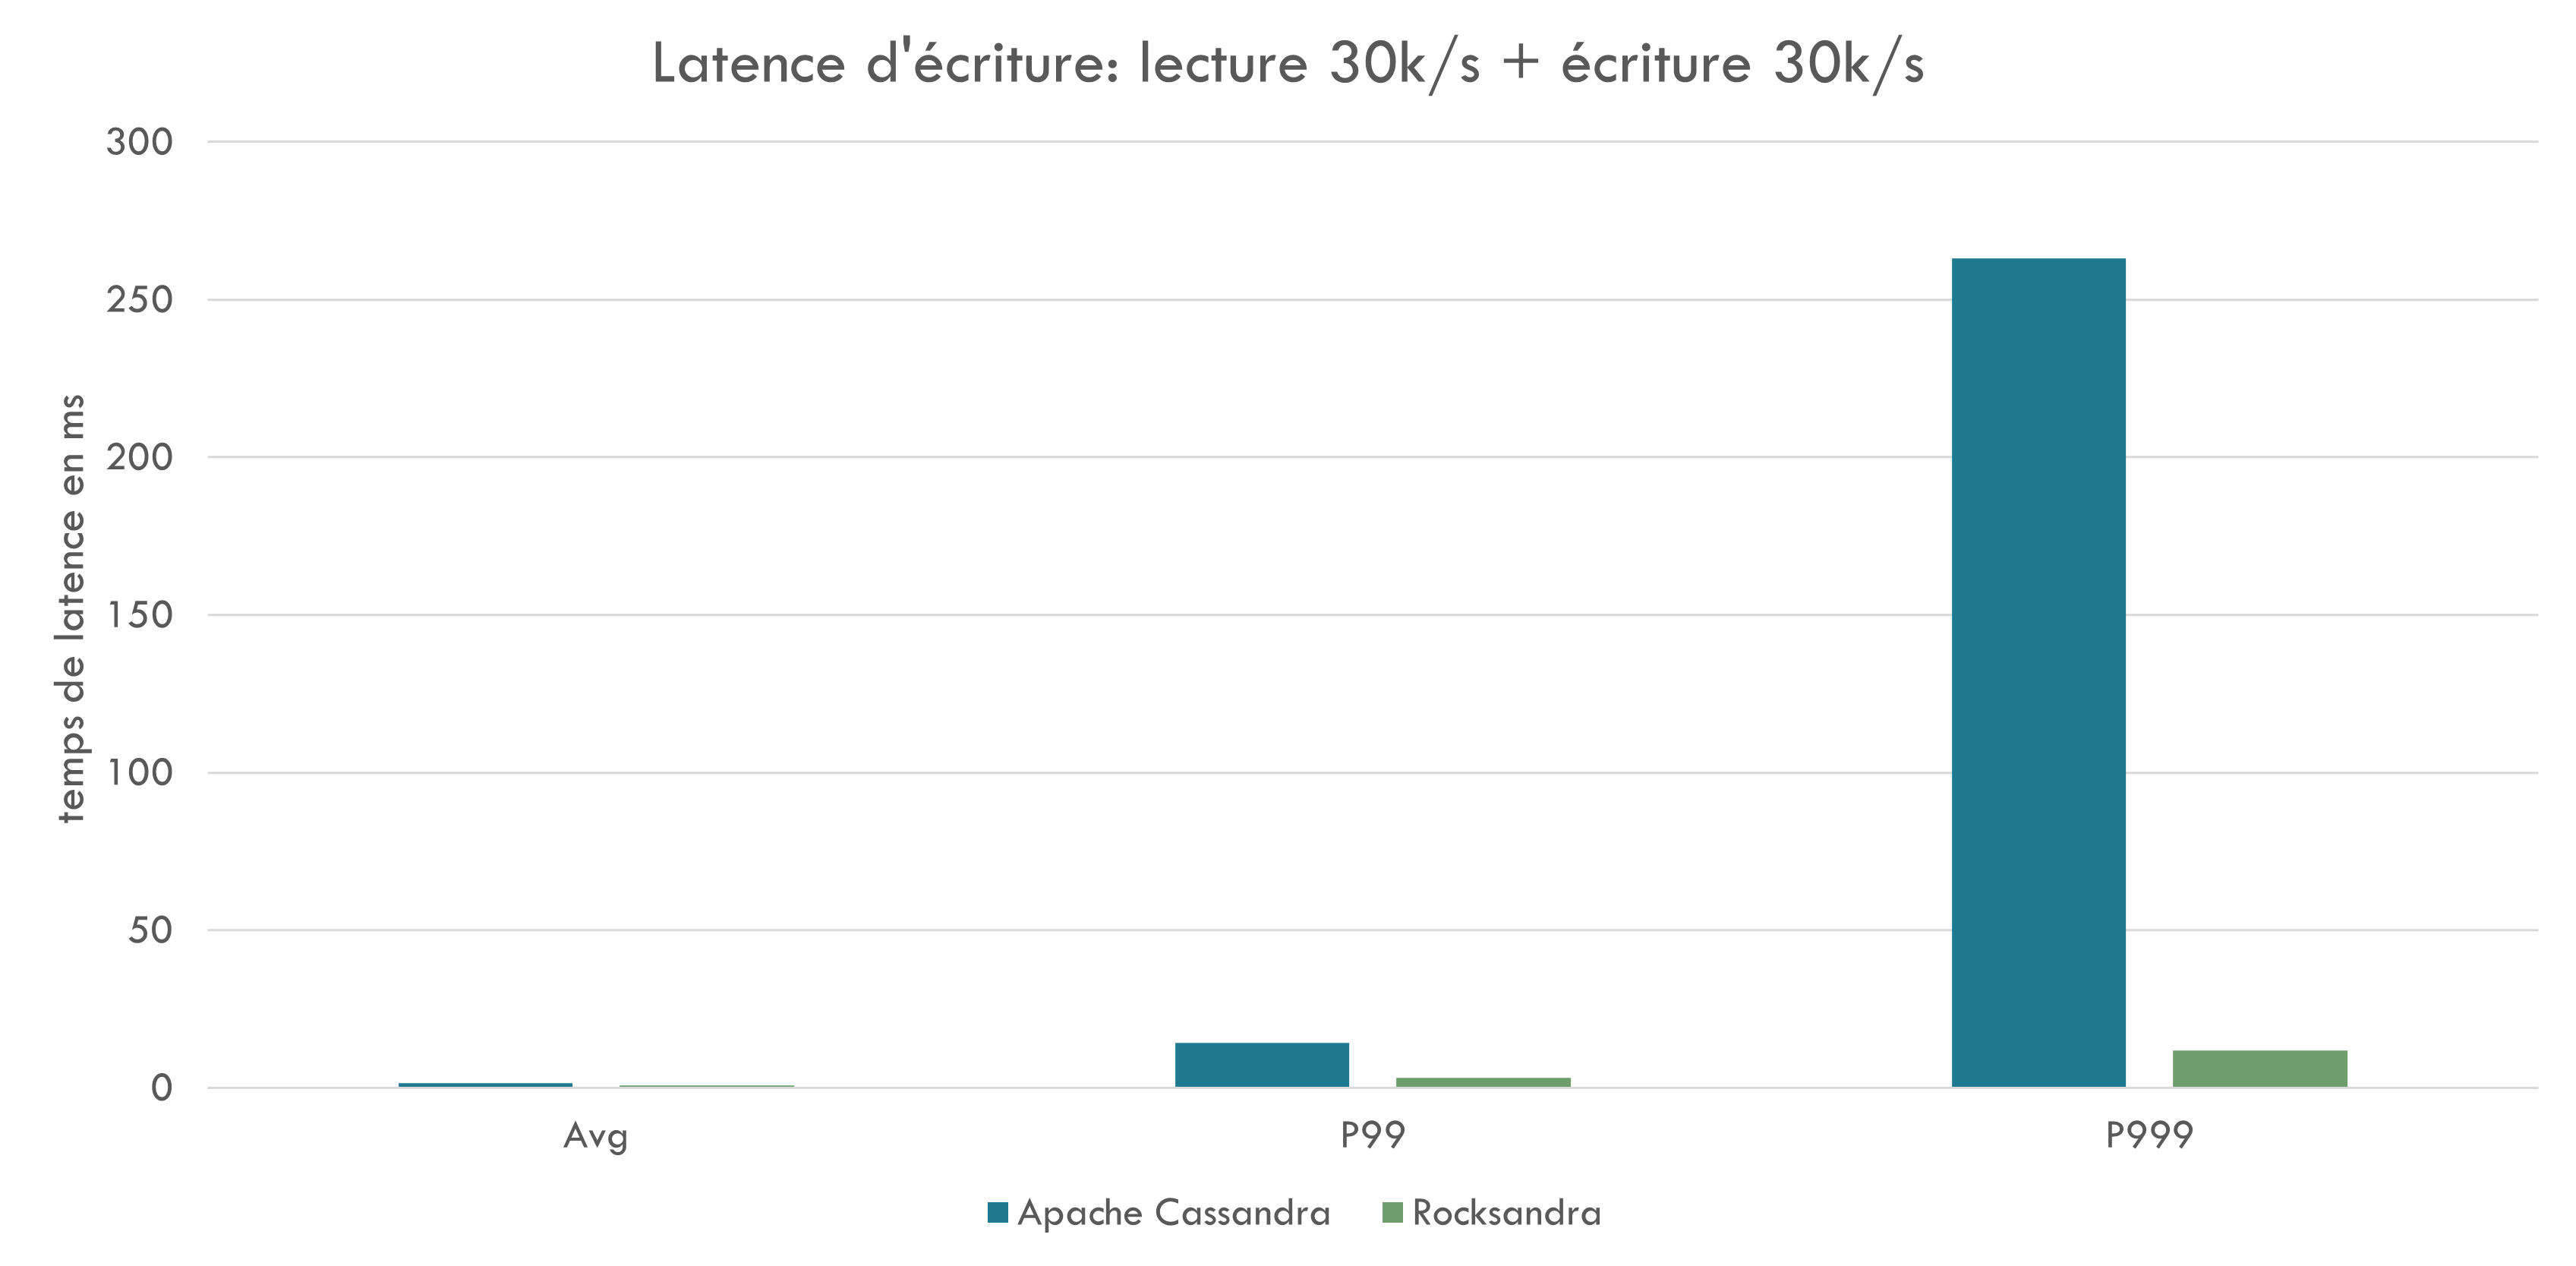
\includegraphics[width=\textwidth]{latence_ecriture}
\end{center}
\begin{center}
	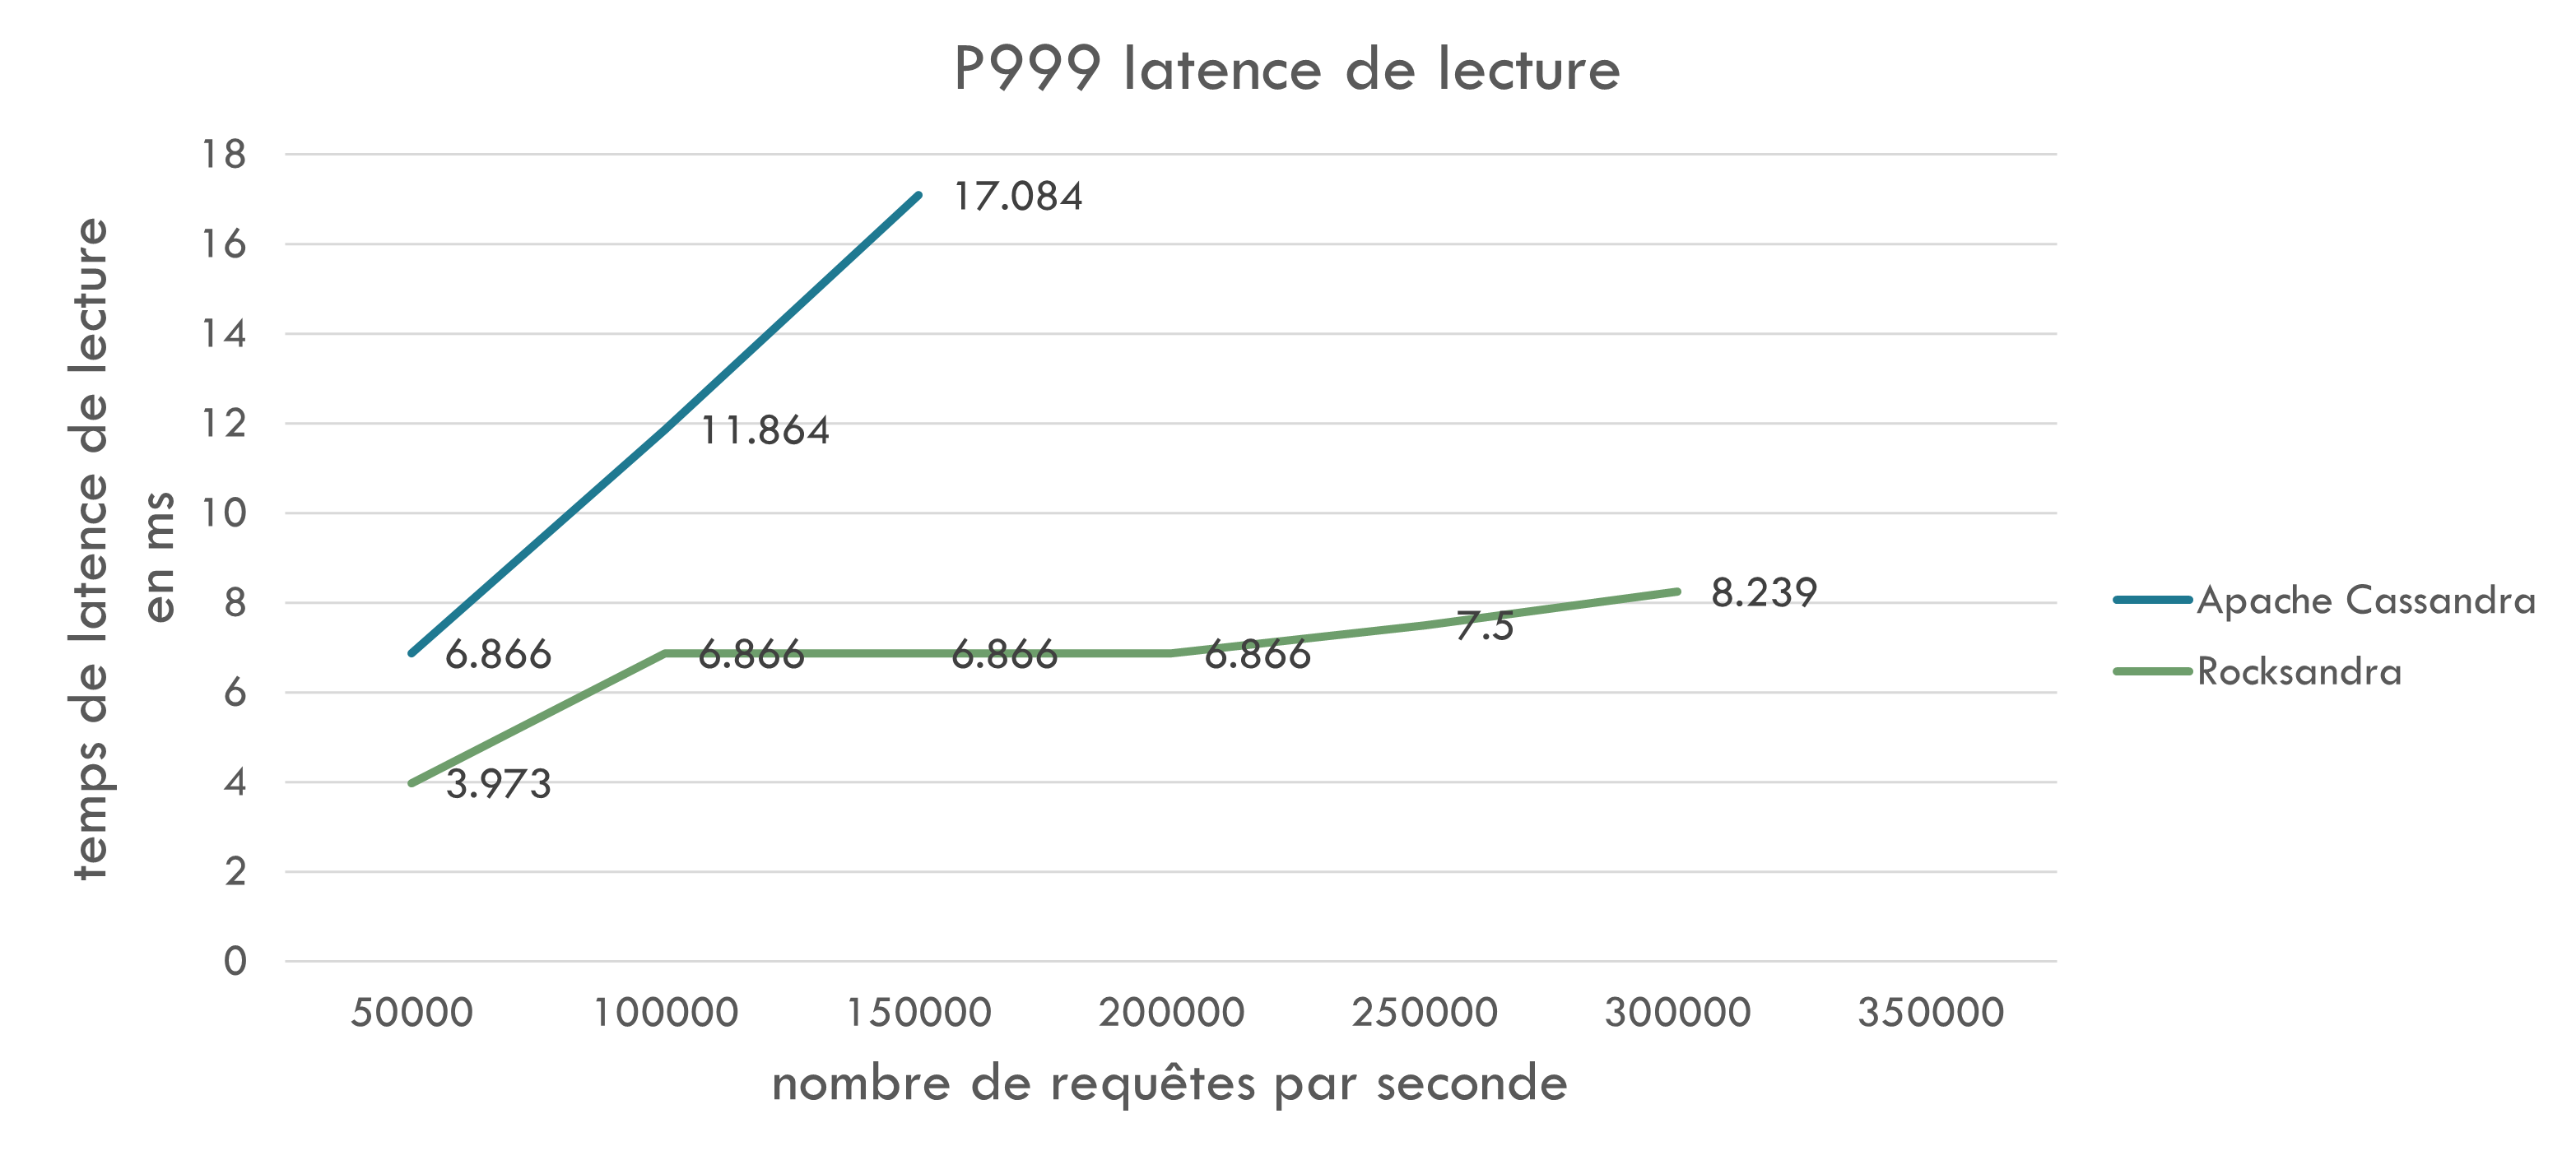
\includegraphics[width=\textwidth]{p999}
\end{center}
\section{Utilisation dans l'industrie}
\begin{center}
	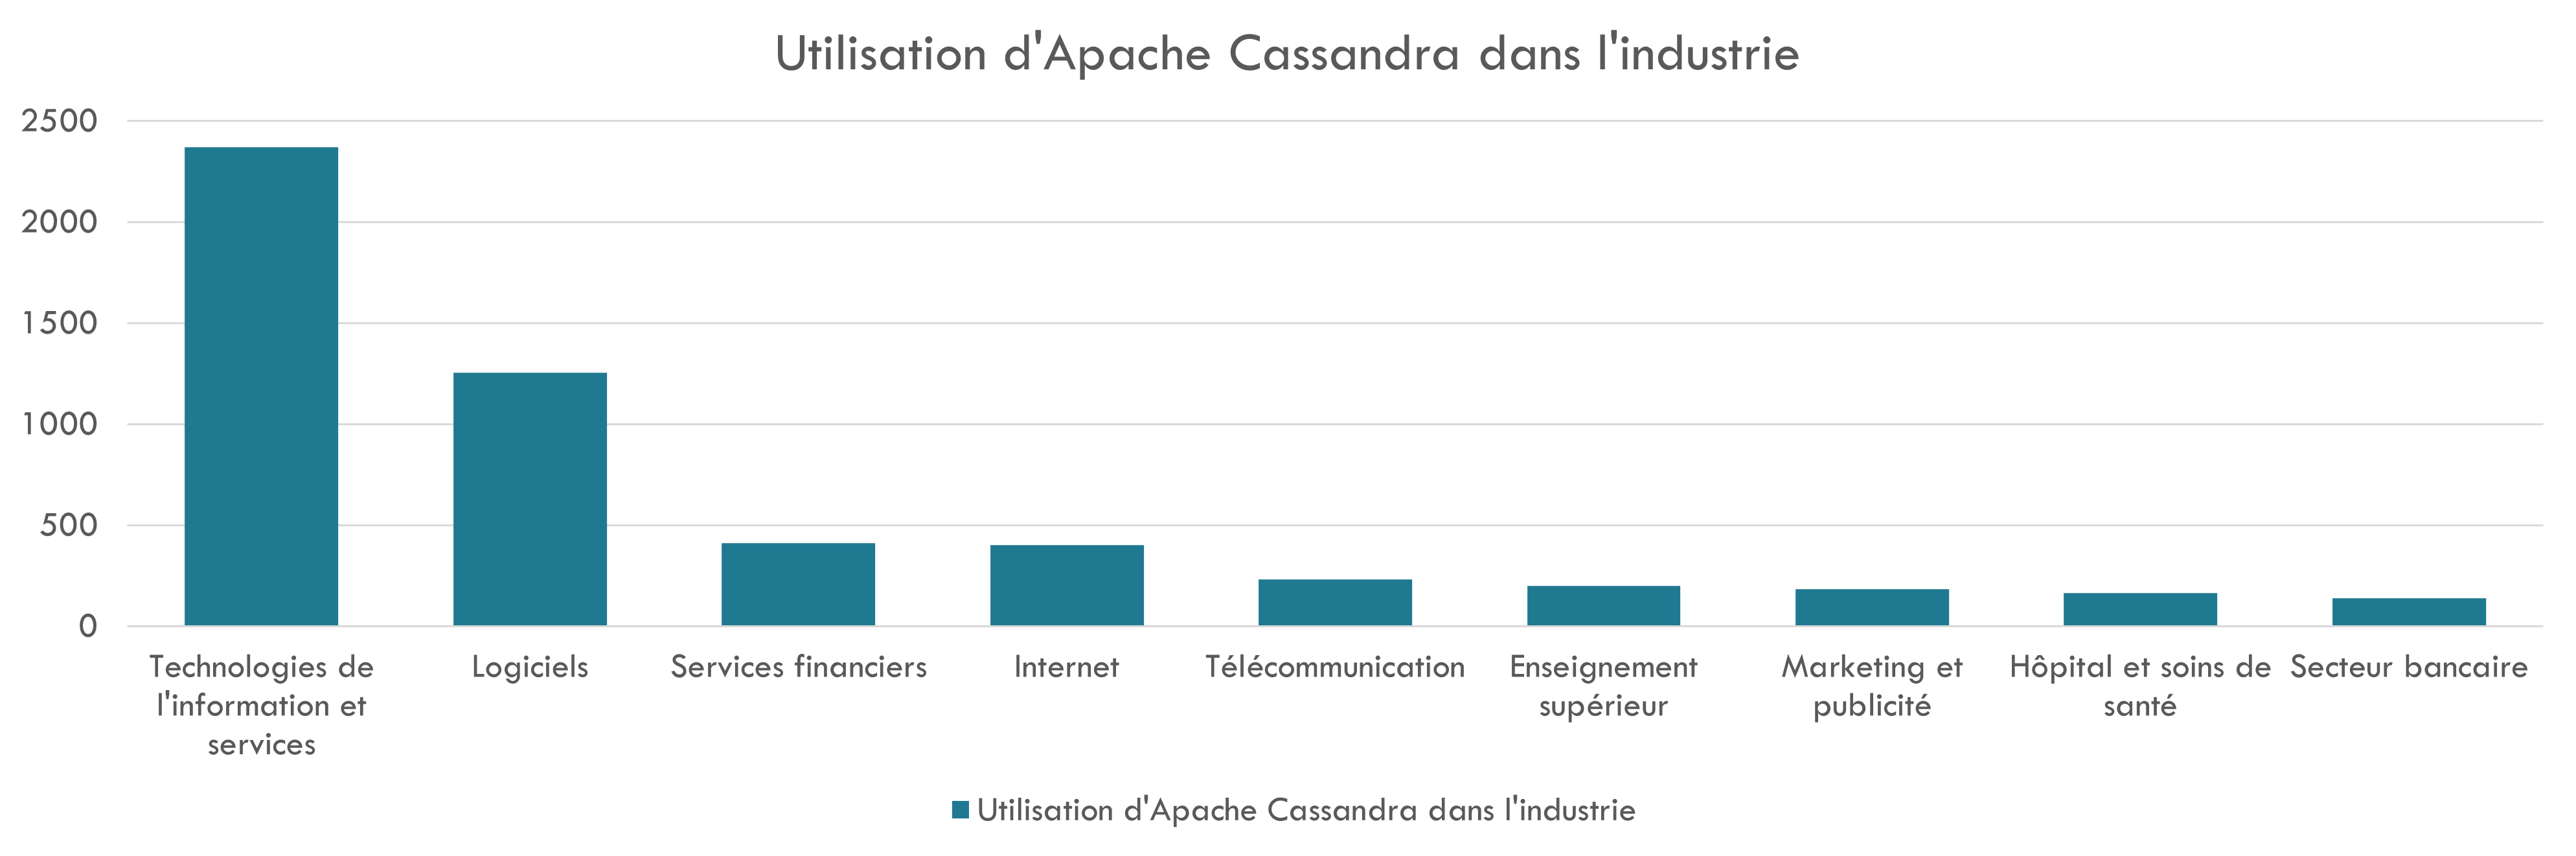
\includegraphics[width=\textwidth]{utilisation}
\end{center}
Depuis sa création en 2008, Cassandra est devenue une technologie populaire dans de nombreux secteurs industriels, notamment le commerce électronique, les réseaux sociaux, les services financiers, la santé, les télécommunications et bien d'autres.
\newline
Dans l'industrie du commerce électronique, Cassandra est largement utilisé pour stocker des données sur les produits, les commandes et les clients. Grâce à sa capacité à gérer de gros volumes de données en temps réel, les détaillants peuvent utiliser Cassandra pour fournir des informations précises et à jour sur les produits et les stocks, ainsi que pour traiter rapidement les commandes et les paiements en ligne.
\newline
Dans les réseaux sociaux, Cassandra est utilisé pour stocker des données sur les utilisateurs, les relations sociales et les messages. En raison de sa capacité à évoluer facilement pour gérer des volumes de données en croissance constante, Cassandra permet aux plateformes de réseaux sociaux de gérer des millions d'utilisateurs et des milliards de messages tout en fournissant une expérience utilisateur rapide et sans faille.
\newline
Bien que Cassandra soit largement utilisée dans de nombreux secteurs industriels, elle n'est pas très répandue dans le secteur bancaire en raison de ses exigences en matière de sécurité, de transaction ACID et de complexité de l'architecture de données. Les banques préfèrent souvent des solutions de base de données traditionnelles et éprouvées qui répondent à leurs exigences spécifiques.
\begin{thebibliography}{widest entry} 
 \bibitem[1]{cite_key1} Instagram post: 
 \href{https://instagram-engineering.com/open-sourcing-a-10x-reduction-in-apache-cassandra-tail-latency-d64f86b43589}{Open-sourcing a 10x reduction in Apache Cassandra tail latency}
 \bibitem[2]{cite_key2} Official documentation: 
 \href{https://cassandra.apache.org/doc/latest/index.html}{Cassandra Documentation}
 \bibitem[3]{cite_key2} Apache Cassandra™ 3.0 Documentation, November 24, 2015
 \bibitem[4]{cite_key2} Cassandra: The Definitive Guide, Eben Hewitt
\end{thebibliography}
\end{document}